\section{Flow in an Open Cavity}
\label{application_cavity}

\subsection{The Extended Problem}

The case of flow in an open cavity is investigated through the lens of the theoretical results developed in section~\ref{center_manifold_derivation}. This was previously studied by \cite{sipp07} in the context of examining the relevance of mean flow stability analysis to frequency prediction and also by \cite{meliga17} for second-order self-consistent approximations. The problem geometry is set up following \cite{sipp07} and is also shown in figure~\ref{fig:cavity_base_param}. The two dimensional computational domain consists of a square cavity with sides of length one and an open channel flow is constructed above the cavity. The top left corner of the cavity is located at $(x,y)=(0,0)$. The open channel has a width of $0.5$ above the cavity and a symmetry boundary condition is applied to the upper boundary of the channel. The inlet of the channel is located at $x=-1.2$ and a uniform inlet veolcity of $u=1.0$ is applied to the inlet. 
A symmetry boundary condition is applied to the lower wall of the channel from $x=-1.2$ to $x=-0.4$ to allow the flow to develop freely from the inlet. A no-slip condition is applied to the lower walls from $x=-0.4$ to $x=1.75$ (including the cavity walls). Thereafter a symmetry condition is applied again at the lower wall from $x=1.75$ to the outlet, located at $x=2.50$. The critical point for the particular geometry is found to be $Re_{c}=4131.33$, which is close to the values of $4140$ and $4114$ reported in \cite{sipp07} and \cite{meliga17} respectively. The spectrum of the flow at the critical point is shown in figure~\ref{fig:cavity_spectrum}. 

The streamwise velocity for the calculated baseflow along with the parameter mode is depicted in figure~\ref{fig:cavity_base_param} . The complex conjugate pair of critical eigenvalues for the baseflow is found to be $\lambda_{c} = \pm7.495i$, which compares well with $\lambda_{c}=\pm7.5i$ reported in \cite{sipp07}. The direct and adjoint critical eigenmodes of the flow are shown in figures~\ref{fig:cavity_flowconfig} and ~\ref{fig:cavity_flowconfig_2} respectively. The complex-conjugated mode is not shown. The modes are normalized as earlier with the direct modes being of unit norm and the adjoint modes are scaled appropriately to maintain biorthogonality. Again, the parameter mode is normalized such that $\zeta^{\dagger}_{0} = \zeta_{0} = 1$.
\begin{figure}
	\centering
	\includegraphics[width=0.49\textwidth]{cavity_baseflow0000}
	\includegraphics[width=0.49\textwidth]{cavity_real_dirmode0000}
	\caption{Streamwise velocity of (top) the stationary base flow for the open cavity flow at $\Rey_{c}=4131.33$ and (bottom) the parameter mode.}
	\label{fig:cavity_base_param}
\end{figure}	

\begin{figure}
	\centering
	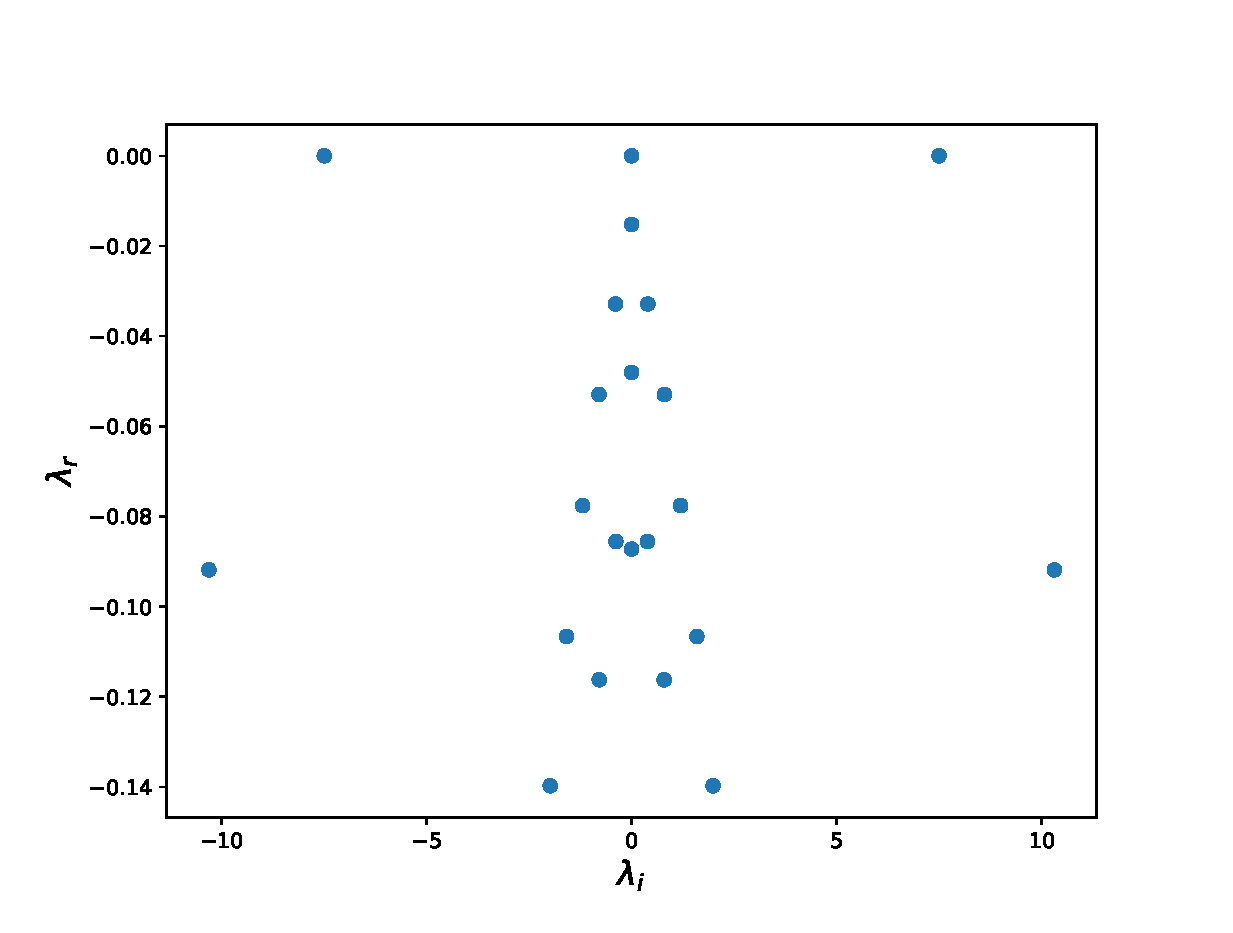
\includegraphics[width=0.49\textwidth]{cavity_spectra}
	\caption{Spectrum of the open cavity flow at the critical point. Note, this is the spectrum of the extended problem which includes the parameter mode located at the origin.}
	\label{fig:cavity_spectrum}
\end{figure}	

\begin{figure}
	\includegraphics[width=0.49\textwidth]{cavity_real_dirmode0001}
	\includegraphics[width=0.49\textwidth]{cavity_imag_dirmode0001}
	\caption{Streamwise velocity of the direct eigenmode. The panels represent the (top) real part and (bottom) imaginary part of the direct critical mode.}
	\label{fig:cavity_flowconfig}
\end{figure}

\begin{figure}
	\includegraphics[width=0.49\textwidth]{cavity_real_adjmode0001}
	\includegraphics[width=0.49\textwidth]{cavity_imag_adjmode0001}
	\caption{Streamwise velocity of the adjoint eigenmode. The panels represent the (top) real part and (bottom) imaginary part of the adjoint critical mode.}
	\label{fig:cavity_flowconfig_2}
\end{figure}

\subsection{Asymptotic Center Manifold}

As done earlier, second order asymptotic approximation of the graph $\mathfrak{h}(\mathbf{x})$ are evalued which requires the evaluation of six restricted resolvent solution fields $\vpfield{y}_{i,j}$. The zero frequency fields that contribute to the mean flow correction ($\vpfield{y}_{0,0}$ and $\vpfield{y}_{1,2}$) are depicted in figure~\ref{fig:cavity_resolvents_zero} while the oscillatory resolvent fields $\vpfield{y}_{0,1}$ and $\vpfield{y}_{1,1}$ are depicted in figures~\ref{fig:cavity_resolvents_oscillatory_real} and \ref{fig:cavity_resolvents_oscillatory_imag}. The corresponding complex conjugated fields ($\vpfield{y}_{0,2}$ and $\vpfield{y}_{2,2}$) are not displayed.
\begin{figure}
	\centering
	\includegraphics[width=0.49\textwidth]{cavity_real_resmode0000}
	\includegraphics[width=0.49\textwidth]{cavity_real_resmode0004}
	\caption{Streamwise velocity components of the restricted resolvent solutions for the open cavity flow corresponding to the zero frequency fields (top) $\vpfield{y}_{0,0}$ and (bottom) $\vpfield{y}_{1,2}$ for the open cavity flow case.}
	\label{fig:cavity_resolvents_zero}
\end{figure}

\begin{figure}
	\centering
	\includegraphics[width=0.49\textwidth]{cavity_real_resmode0001}
	\includegraphics[width=0.49\textwidth]{cavity_real_resmode0003}
	\caption{The panels depict the real part of the streamwise velocity components of (top) $\vpfield{y}_{0,1}$ and (bottom) $\vpfield{y}_{1,1}$ with angular frequencies equal to the imaginary parts of $\lambda_{c}$ and $2\lambda_{c}$.}
	\label{fig:cavity_resolvents_oscillatory_real}
\end{figure}
\begin{figure}
	\centering
	\includegraphics[width=0.49\textwidth]{cavity_imag_resmode0001}
	\includegraphics[width=0.49\textwidth]{cavity_imag_resmode0003}
	\caption{The panels depict the imaginary part of the streamwise velocity components of (top) $\vpfield{y}_{0,1}$ and (bottom) $\vpfield{y}_{1,1}$ with angular frequencies equal to the imaginary parts of $\lambda_{c}$ and $2\lambda_{c}$.}
	\label{fig:cavity_resolvents_oscillatory_imag}
\end{figure}

 The center-manifold amplitude equation can be easily obtained once the resolvent fields have been calculated.  Replacing $x_{0},x_{1},x_{2}$ with $\eta,x,x^{*}$, one obtains the following equation for $\dt{x}$,
\begin{equation}
	\label{cavity_numerical_amplitude_eqn_x1_p1}
	\begin{aligned}
			\dt{x} =& +[7.495i]x \\
			%
			& + [(11.72 - 6.618i)\times10^{-2}]\eta^{2} \\
			%
			& + [(8.345 + 7.238i)\times10^{-1}]\eta x \\ 
			%
			& - [(1.544 - 5.471i)\times10^{-2}]\eta x^{*}  \\
			%
			& + [(18.42 - 4.701i)\times10^{-1}] x^{2} \\
			%
			& + [(2.268 - 3.955i)\times10^{+0}] x^{*}x \\
			%
			& + [(1.007 + 4.994i)\times10^{-1}](x^{*})^{2} \\
			%
			& + [(9.656 - 5.478i)\times10^{-2}]\eta^{3} \\
			%
			& + [(3.188 + 2.514i)\times10^{-1}]\eta^{2}x \\
			%
			& - [(7.922 - 2.635i)\times10^{-2}]\eta^{2}x^{*}  \\
			%
			& + [(12.94 - 6.695i)\times10^{-1}]\eta x^{2}  \\
			%
			& + [(0.898 - 1.946i)\times10^{+1}]\eta x^{*}x \\
			%
			& + [(2.234 - 2.946i)\times10^{-1}]\eta(x^{*})^{2} \\
			%
			& - [(3.701 - 3.134i)\times10^{+0}]x^{3} \\
			%
			& - [(5.744 - 3.425i)\times10^{+2}](x^{*}x)x \\
			%
			& - [(9.844 - 3.445i)\times10^{+1}](x^{*}x)x^{*} \\
			%
			& - [(4.613 - 6.681i)\times10^{+0}](x^{*})^{3}.
		\end{aligned}
\end{equation}
In contrast to the reduced equation obtained for the flow across a cylinder, there are no obvious symmetries in the problem and therefore extremely small terms are not obtained for the reduced equations of the open cavity flow. Additionally, the center-manifold amplitude equations are now inhomogeneous, since the terms of the type $\eta^{2}, \eta^{3}$ now have a non-zero coefficient.  The comparison of the angular frequencies obtained through the center manifold equations with those of the full system is shown in figure~\ref{fig:cavity_limit_cycle_frequency}. The system has an interesting behavior past the bifurcation point wherein, initially the system evolves with an angular frequency close to that of the critical mode at bifurcation, clearly indicating the continuation of the system dynamics along the center manifold. However, around $Re=4550$ the non-linear frequencies change abruptly. The spectrum at bifurcation shown in figure~\ref{fig:cavity_spectrum} indicates that the new angular frequency is likely related to the isolated subcritical mode of the system, implying the occurence of mode switching. Obviously the mode switching behaviour can not be captured by the center-manifold amplitude equations since the information regarding the isolated subcritical mode is not captured by the reduced system of equations. Nonetheless, before the mode switching occurs, the angular frequency predicted by the reduced equations agrees very well with those obtained from the full system. 
\begin{figure}
	\centering
	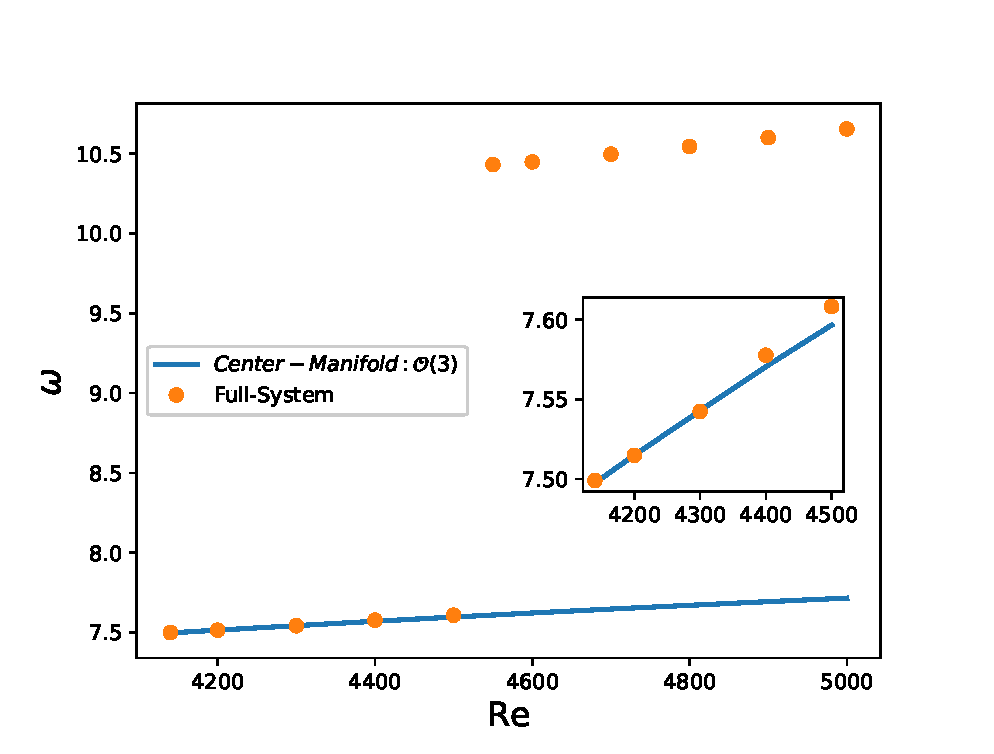
\includegraphics[width=.49\textwidth]{cavity_center_manifold_omega}
	\caption{Comparison of the linear and non-linear angular frequencies of the full system and the center-manifold amplitude equations for the open cavity flow. The frequencies before the mode switching are in good agreement with each other}
	\label{fig:cavity_limit_cycle_frequency}
\end{figure}

The equation for the Landau model and the slow phase variation are obtained as 
\begin{align}
	\label{cavity_landau_eqn_1}
		\dfrac{d|A|^{2}}{dt} =& 2\times[0.834\eta + 0.319\eta^{2}] |A|^{2} - 1148.78|A|^{4}, \\
	\label{cavity_landau_eqn_2}
	\dfrac{d\phi}{dt} =& [0.7238\eta + 0.2514\eta^{2}]  + 342.47|A|^{2},
\end{align}
with the combined Stuart-Landau equation being
\begin{eqnarray}
	\label{cavity_stuart_landau_eqn}
	\begin{split}
		\dt{A} 					=& [(0.834 + i0.7238)\eta + (0.319 + i0.2514)\eta^{2}] A \\
										& - \frac{1}{2}[1148.78 - i684.94]|A|^{2}A.
	\end{split}
\end{eqnarray}

This presents a rather interesting case for the mathematical modeling of fluid flows since the mode switching behavior is not captured by the center-manifold nevertheless the flow has a distinct angular frequency and no sign of chaotic behavior clearly suggesting the evolution of the dynamics in some low dimensional subspace. The relaxation of the assumption of critical eigenvalues of the dynamic subspace leads naturally to the invariant manifold theory however, the application of this theory requires the existence of a spectral gap between the eigenvalues of the dynamic and driven subspaces \citep{chicone06}. The spectrum plotted in figure~\ref{fig:cavity_spectrum} indicates that if one considers the eigenmodes corresponding to the two isolated eigenvalues as part of the dynamic subspace the spectral gap assumption is not fullfilled. The mathematical modeling in such a scenario clearly requires a further refinement of the underlying assumptions. 

Finally, a few comments may be made with regards to the comparison of the current work with the weakly non-linear analysis that is common in hydrodynamics. Despite claims of equivalence \citep{fujimara91} of the final Landau equations, the formal procedure for evaluation of solution is quite different for the two methods. Nonetheless, given that both methods are applied close to the bifurcation point and are trying to capture essentially the same physics, one would expect that the results of the two methods would indeed be similar. Indeed some of the coefficients of the Stuart-Landau equation obtained for the case of the cylinder are similar to those reported in the literature using weakly nonlinear analysis \citep{sipp07}. However, some differences do seem to arise. In the current work, the coefficient of the linear term $A$ is obtained up to quadratic order in $\eta$. The author is unaware of any work utilizing weakly non-linear analysis for the current cases that reports such a quadratic variation. Differences also arise in the coefficient of the cubic term $|A|^{2}A$. The work of \cite{sipp07} contains a linear dependence on the parameter for this term while in the current investigation the cubic saturation term is devoid of any such dependence. Formally, a term of the type $\eta|A|^{2}A$, when viewed in the current framework would be a fourth order term since the parameter perturbation is treated through the term $x_{0}$ which is just another mode amplitude. These are structural differences in the solutions which no doubt partly arise due to the distinct treatment of the parameter variation. Such structural differences in the two methods could be an example of the claims made in \cite{fujimara91} that high order evaluations may be required to achieve exact equivalences. A systematic comparison, including evaluation of higher orders, would be required to tease out such differences. 

\section{Conclusion}
\label{conclusion}
A center-manifold reduction for the Navier--Stokes equation is derived with the extension of the system to include the trivial parameter evolution equation. This inclusion however enlarges the critical subspace in a non-trivial manner. The system is then reformulated to bring it to an appropriate form and the application of center-manifold theorem leads to a graph equation for the reformulated system. The graph equation is a representation of the infinite dimensional stable subspace that is driven by the dynamics in the critical subspace. The equation is solved asymptotically and expressions for the asymptotic solutions are obtained, which finally result in a set of equations for center-manifold amplitude equations for the critical eigenvectors. The derivation is essentially agnostic to the dimension of the critical subspace however, the number terms required for the asymptotic evaluation rises rapidly with increasing critical subspace dimension. While the derivation is set in the context of the Navier--Stokes, the methodology is more general and equations~\eqref{general_second_order_expression} and \eqref{general_higher_order_expression} point to the essential structure of the asymptotic solutions of the graph equation that may be obtained for other infinite-dimensional problems. 

The proposed method with system extension is of particular relevance when considering center-manifold reduction for problems that have been perturbed away from the bifurcation point and is a formal way to incorporate parameter perturbations within the asymptotic approximations of the graph equation thereby negating the need for a double asymptotic expansion or an apriori assumption of the normal form of the reduced dynamics.

The derivation is then applied to two cases - the case of the Hopf bifurcation of a cylinder wake and flow in an open cavity resulting in the reduced center-manifold amplitude equations from which, the Stuart-Landau equations are derived. The results from the reduced equations provide a good prediction for the frequencies of the full system close to the bifurcation point. In particular, the linearized eigenvalue variation is predicted up to fourth order in $\eta$ for the case of the cylinder flow and it is found to match well with the spectra calculation of the full system at different Reynolds numbers. The case of flow in an open cavity has interesting dynamics with clear evidence of mode switching at a certain parameter value. This mode switching behavior can not be captured within the bounds of center-manifold theory. Nevertheless, the frequency prior to the mode switching is indeed predicted well by the center-manifold reduction of the extended system.

\FloatBarrier


